\section{Results}

\subsection{Quantitative Results}

\subsubsection{GMM}

All proposed methods are able to increase the main network's accuracy and validation accuracy.
Also, the accuracy of the verifier network is increased.
It is interesting to note that all methods do not decrease the l2-error of the distortion,
yet the cross-entropy, for most is decreased.

For a larger number of samples, the data set cross-entropy quickly becomes infeasible
due to floating point precision errors, even with overflow measures in place.

Although, it is important to remember that the loss function used in the optimization process
is a composite loss from the proposed loss between the statistics
and the original cross-entropy loss used in the optimization of the neural network.
\[
    r_{stats} \loss(\set A, \set B) + r_{crit}\loss_{crit}(\set B, y_{\set B})
\]
Since the original criterion loss alone already performs quite good, 
it can be said that the proposed losses act as a kind of regularization 
by incorporating more knowledge about the target data distribution that prevent overfitting
of the source data set.
A comparison of the results for the case $r_{crit}=0$ can be found in table \ref{tab:gmm_results_raw}

The results shown in table \ref{tab:gmm_results_raw} confirm the assumption that the methods alone 
- without any class information - are not able to achieve good results.

In this scenario, two methods, namely NN CC and RP CC seem to give even better generalization scores 
(validation and verifier accuracy) than when the original cross-entropy loss is included.
Although it is hard to explain the lower cross-entropy loss when leaving out the loss that
is designed to minimize said loss.
It is important to note that scores can fluctuate a fair amount and more experiment runs are
necessary to give a clearer picture.

\begin{table}[!htbp]
\centering
\footnotesize
\pgfplotstabletypeset[
results,
gmm,
display columns/0/.style={column name=\textbf{Baseline}, column type=l, string type},
]{figures/reconstruction_GMM_baseline.csv}
\caption{GMM baseline scores}
\label{tab:gmm_baseline}
\end{table}

\begin{table}[!htbp]
\centering
\footnotesize
\pgfplotstabletypeset[
results,
gmm,
every row 6 column 1/.style={highlight},
every row 8 column 1/.style={highlight},
every row 10 column 1/.style={highlight},
every row 11 column 1/.style={highlight},
every row 7 column 2/.style={highlight},
every row 4 column 3/.style={highlight},
every row 8 column 4/.style={highlight},
every row 8 column 5/.style={highlight},
]{figures/reconstruction_GMM_results.csv}
\caption{Metrics on reconstruction results after 100 optimization epochs on GMM data set}
\label{tab:gmm_results}
\end{table}

\begin{table}[!htbp]
\centering
\footnotesize
\pgfplotstabletypeset[
results,
gmm,
every row 1 column 1/.style={highlight},
every row 7 column 2/.style={highlight},
every row 7 column 3/.style={highlight},
every row 4 column 4/.style={highlight},
every row 7 column 5/.style={highlight},
]{figures/reconstruction_GMM_results_raw.csv}
\caption{Metrics on reconstruction results after 100 optimization epochs for $r_\text{crit}=0$ on GMM data set}
\label{tab:gmm_results_raw}
\end{table}


When reviewing the trajectories of the scores, many of the methods show that soon after
 the loss passes a reference value - the same loss calculated on a batch of 
unperturbed data - the l2-error is seen to increase. This can be seen in figure \ref{fig:metrics_GMM_l2_increase}.

\begin{figure}[!htbp]
    \centering
    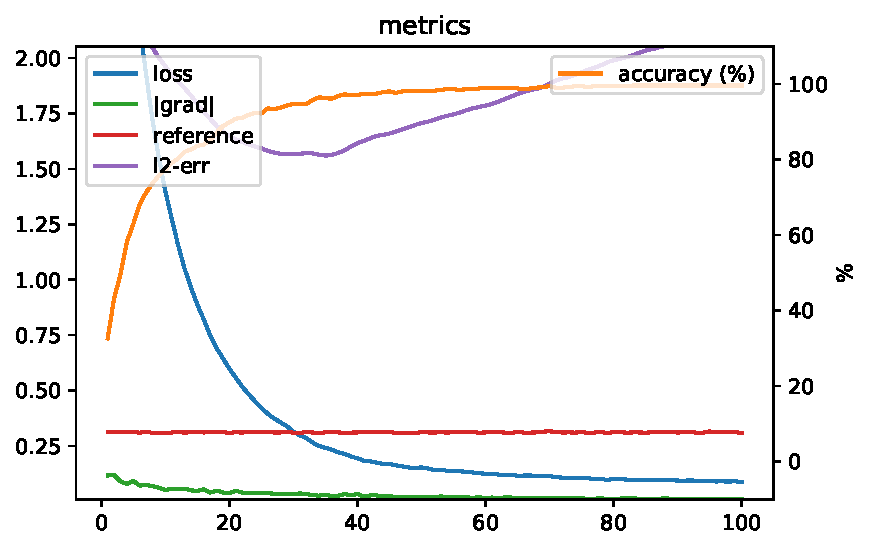
\includegraphics[width=0.7\textwidth]{figures/reconstruction_GMM_NN_ALL_metrics.pdf}
    \caption{Plot of optimization metrics of method NN ALL \\on the GMM data set}
    \label{fig:metrics_GMM_l2_increase}
\end{figure}

\subsubsection{MNIST}


The distortion factor ($\kappa = 0.2$) on the MNIST data set was chosen to be fairly strong.
After distortion, the overall accuracies drop from 97-99\% to near random guesses $\frac 1 C \approx 10\%$
as seen in table \ref{tab:mnist_baseline}.
The results for the reconstruction task for all methods on the MNIST data set is depicted in table \ref{tab:mnist_results}.
The criterion (CRITERION) alone gives leads to good results on the main network, but fails to generalize when tested on a secondary network.
This shows that the reconstruction is being heavily biased by what the neural network deems to be "correct" images, 
yet these features might not be robust in the sense that they don't correspond to features we as humans might make out.
The hardly improved generalization score of NN, where additionally the second-to-last layer is incorporated seems to confirm
the network's bias in the optimization procedure. Only by taking into account all layers of the neural network (NN ALL), an
improvement in the verifier accuracy can be seen.
The randomly initialized neural network (RANDOM NN) does not add any significant improvement - it seems as though it is
not able to capture any useful information about the data set.
Random projections (RP) is able to add an additional amount of regularization that is seen in the generalization scores.
Combining the methods (COMBINED) seems to merit overall good scores which can be verified in image quality.


\begin{table}[!htbp]
\centering
\footnotesize
\pgfplotstabletypeset[
results,
images,
display columns/0/.style={column name=\textbf{Baseline}, column type=l, string type},
]{figures/reconstruction_MNIST_baseline.csv}
\caption{MNIST baseline scores}
\label{tab:mnist_baseline}
\end{table}

\begin{table}[!htbp]
\centering
\footnotesize
\pgfplotstabletypeset[
results,
images,
every row 11 column 1/.style={highlight},
every row 11 column 2/.style={highlight},
every row 11 column 3/.style={highlight},
every row 11 column 4/.style={highlight},
every row 5 column 5/.style={highlight},
every row 6 column 6/.style={highlight},
]{figures/reconstruction_MNIST_results.csv}
\caption{Metrics on reconstruction results after 100 optimization epochs on MNIST data set}
\label{tab:mnist_results}
\end{table}


Here, it is important to note that the l2-error and the PSNR-score do not improve after the reconstruction task is performed.
Contrasting these findings with the qualitative results shown in figure \ref{fig:MNIST_Images} of the appendix, 
leads to the conclusion that these scores are not indicative of proper image quality.
These scores rely on per-pixel comparisons and the reconstruction network may introduce shifts in the final image
that can greatly disrupt the score of these metrics.
The SSIM-score seems to be more robust metric in this regard that correlates better with perceived image quality.





\subsubsection{CIFAR10}

The CIFAR10 data set is a more complex data set compared to the previous two.
The objects of interest have greatly varying backgrounds and are shown from numerous different angles.
The learned feature representations have to be able to filter out the noise from the signal more than in
the previous data sets.
The network for this data set is of a deeper (34 layers) architecture,
the learned feature representations seem to be more robust and correlate more with the verifier network.
Comparing the results of the methods that use the representations of the main network (NN, NN ALL)
to the randomly initialized network (RANDOM NN), it can be said that a good feature representation is necessary.
Random projections do not perform well for this task, their design is too simple for this complex task.

\begin{table}[!htbp]
\label{tab:cifar10baseline}
\centering
\footnotesize
\pgfplotstabletypeset[
results,
images,
display columns/0/.style={column name=\textbf{Baseline}, column type=l, string type},
]{figures/reconstruction_CIFAR10_baseline.csv}
\caption{CIFAR10 baseline scores}
\end{table}

\begin{table}[!htbp]
\label{tab:cifar10results}
\centering
\footnotesize
\pgfplotstabletypeset[
results,
images,
every row 2 column 1/.style={highlight},
every row 4 column 1/.style={highlight},
every row 3 column 2/.style={highlight},
every row 4 column 3/.style={highlight},
every row 3 column 4/.style={highlight},
every row 3 column 5/.style={highlight},
every row 3 column 6/.style={highlight},
]{figures/reconstruction_CIFAR10_results.csv}
\caption{Metrics on reconstruction results after 100 optimization epochs for CIFAR10}
\end{table}





Of the methods using neural networks, it seems as though NN ALL has the overall best performance.
The difference between the class-conditional version (NN ALL CC) and the original formulation is negligible
and from inspecting qualitative results seems to be slightly worse.
A reason as to why the class-conditional variants don't seem to increase performance could be that 
the network is already complex enough to "split" the signal into distinct enough paths so that adding
a class-conditional formulation does not add more context.
It might even be more of a hindrance, because of the high variance in image statistics
from one image to another due to the background "noise".
Since the class-conditional formulation groups inputs by their respective classes, 
and the batching is done randomly (independently of the classes), it might happen, that one iteration
might contain a batch with only few samples of one class or where one grouped class simply batch happens
to display unusual statistics (by, for example, all having red backgrounds).
This in turn can lead to a spike in the loss which can lead to large gradients that corrupt the optimization.
Increasing the batch size can help mitigate this problem as the statistics become more stable.
Although, still, if the loss that comes from the difference in the mean between the source and the target 
is plotted for each layer, as seen in \ref{fig:layer_losses}, it can be seen that while the
normal formulation is able to minimize statistics over all layers relatively uniformly,
the class-conditional variation struggles with the few earlier layers.
These exhibit higher losses that the reconstruction network is not able to minimize.
Possible solutions to this problem could be to simply increase the batch size;
to have the losses be weighted by their layer; or to formulate a hybrid approach, which
only uses class information in the later layers.

\begin{figure}
    \centerline{
    \hspace*{6mm}
    \begin{minipage}{0.6\textwidth}
    \caption*{NN ALL}
    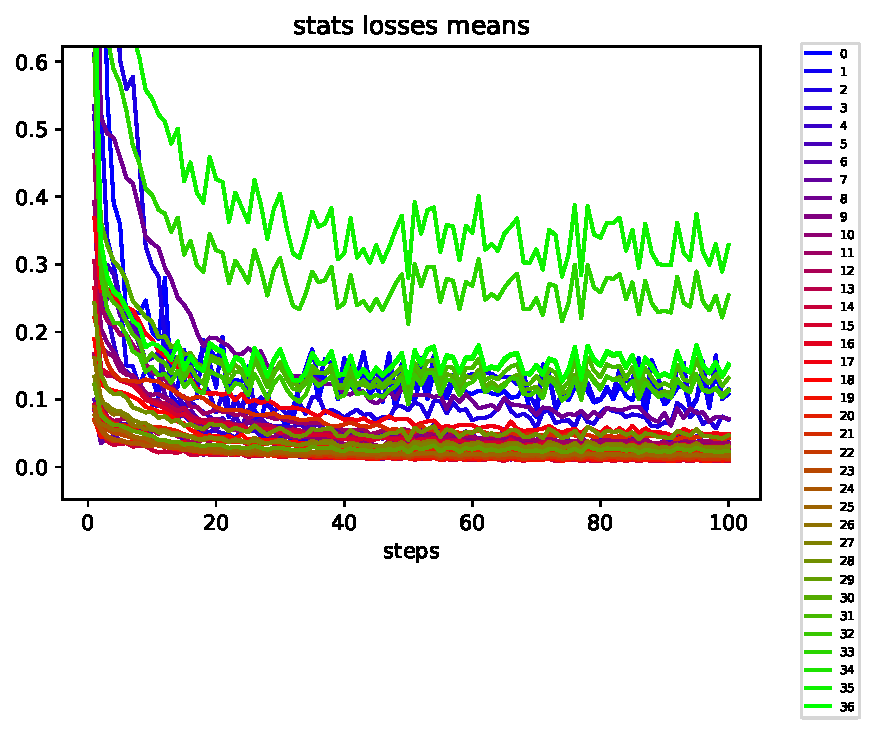
\includegraphics[
    width=\textwidth, 
    trim={0 0 0 0.6cm}, clip,
    ]{figures/reconstruction_CIFAR10_NN_ALL_metrics_stats_losses_means.pdf}
    \end{minipage}%
    \begin{minipage}{0.6\textwidth}
    \caption*{NN ALL CC}
    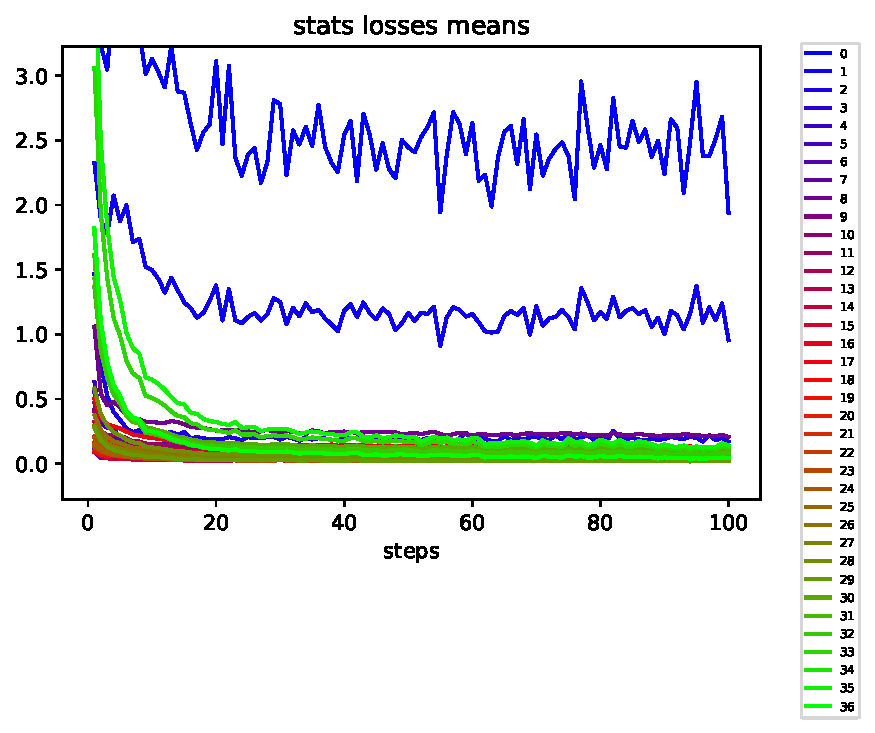
\includegraphics[
    width=\textwidth,
    trim={0 0 0 0.6cm}, clip,
    ]{figures/reconstruction_CIFAR10_NN_ALL_CC_metrics_stats_losses_means.pdf}
    \end{minipage}
    }
    \caption{Loss coming from the difference in mean batch-statistics plotted per layer. 
    Lighter colors correspond to later layers in the network. \textit{Layer 0} is the input itself.}
    \label{fig:layer_losses}
\end{figure}



Conclusion:...
Incorporating the non-linearity ReLU in the random projections (RP ReLU), in general, 
does not seem to lead to any notable differences of the performance.



\subsection{Hyperparameter-influence}


In the following, the influence of various hyperparameter settings on the reconstruction outcome is studied.
A grid search is performed on:
\begin{flalign*}
    s_\text{width} &\in \{4, 8, 16\} &\\
    s_\text{depth} &\in \{4, 8, 16\} \\
    n_{\set B} &\in \{128, 512, 1024, 2048\} \\
\end{flalign*}

Every run depicts a hyperparameter setting ($s_\text{width} s_\text{depth}  n_{\set B}$) of the Cartesian product
of all possible values shown above.

The results are depicted in \ref{fig:rec_hyperparameter_search}.

The influence of $n_{\set B}$ on the outcome is quite clear, the width and the depth of the reconstruction
network is not. In fact, it might even seem as though an increase in complexity of the model is rather
detrimental to the scores.

The findings are solidified in figure \ref{fig:rec_hyperparameter_heatmap}, where a correlation heat map is given
between the parameters and the scores is given.

While $n_{\set B}$ is clearly positively correlated for all scores (except for the l2-error, though here,
a lower score is better), the other parameters show an almost inverse effect on the outcome.






\begin{figure}[!htbp]
\centering
    \centerline{
    \hspace*{6mm}
    \begin{minipage}{0.6\textwidth}
    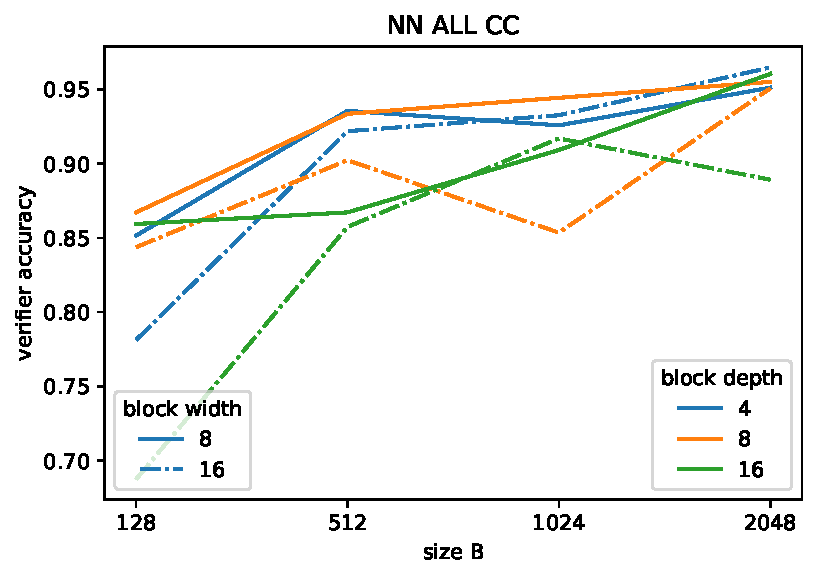
\includegraphics[width=\textwidth]{figures/comparison_CIFAR10_verifier_accuracy_NN_ALL_CC.pdf}
    \end{minipage}%
    \begin{minipage}{0.6\textwidth}
    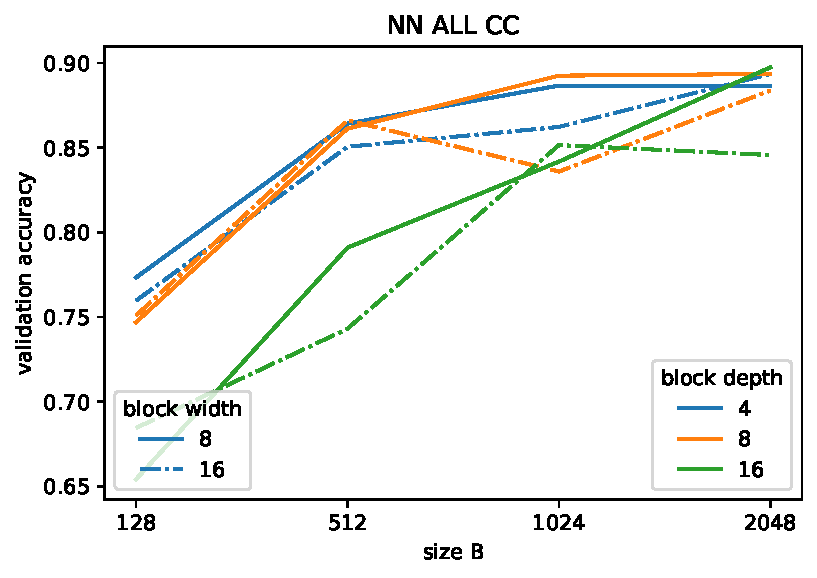
\includegraphics[width=\textwidth]{figures/comparison_CIFAR10_validation_accuracy_NN_ALL_CC.pdf}
    \end{minipage}
    }
\caption{Reconstruction Results for multiple hyperparameter settings on CIFAR10. 
Every data point depicts the end-results after 100 epochs.}
\label{fig:rec_hyperparameter_search}
\end{figure}


\begin{figure}[!htbp]
\centering
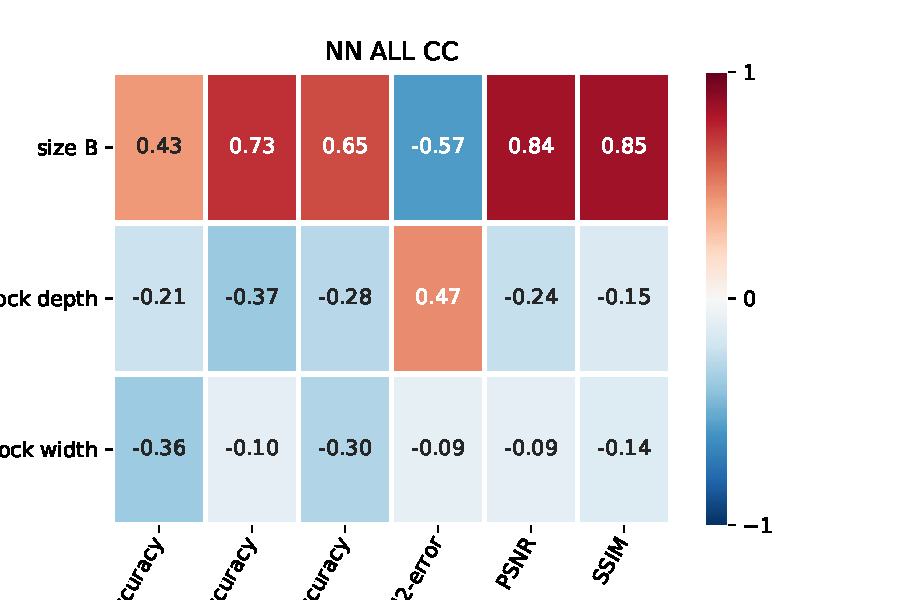
\includegraphics[width=0.7\textwidth]{figures/comparison_CIFAR10_heatmap_NN_ALL_CC.pdf}
\decoRule
\caption{heatmap}
\label{fig:rec_hyperparameter_heatmap}
\end{figure}




















